
\begin{enumerate}


\item If the sum of zeroes of the polynomial $ p\brak x = 2x^2 - k\sqrt2x+1 $ is${\sqrt2} $,then value of k is:
\begin{enumerate}
    \item $ \sqrt{2} $
    \item $2$
    \item $ 2  \sqrt{2} $
    \item $ \frac{1}{2} $
 \end{enumerate}

\item If the roots of the equation $ax^2 + bx + c = 0$,$a \neq 0$ are real and equal, then which of the following relations is true?
\begin{enumerate}    
    \item $a = \frac{b^2}{c}$
    \item $b^2 = ac$                                                                                    \item $ac = \frac{b^2}{4}$
    \item $c = \frac{b^2}{a}$
\end{enumerate}

\item In an A.P., if the first term $a = 7$, $n$th term $a_{n} = 84$, and the sum of the first $n$ terms $s_{n} = \frac{2093}{2}$, then $n$ is equal to:
\begin{enumerate}
    \item $22$
    \item $24$
    \item $23$
    \item $26$
\end{enumerate}

\item The zeroes of a polynomial $x^2 + px + q$ are twice the zeroes of the polynomial $4x^2 - 5x - 6$. The value of $p$ is:
	\begin{enumerate}   
\item $-\frac{5}{2}$
    \item $\frac{5}{2}$
    \item $-5$
    \item $10$
	\end{enumerate}
\newpage
 \item In the given figure, graphs of two linear equations are shown. The pair of these linear equations is:
\begin{figure}[!ht]
\centering
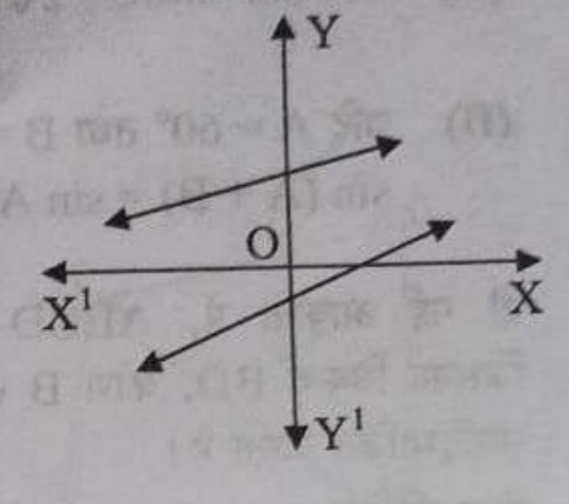
\includegraphics[width=\columnwidth]{figs/Image1.jpg}
\caption{}
\label{fig:enter-label}
\end{figure}
\begin{enumerate}
    \item consistent with a unique solution.
    \item consistent with infinitely many solutions.
    \item inconsistent.
    \item inconsistent but can be made consistent.
\end{enumerate}
\end{enumerate}
